%
% 5-mendez.tex
%
% (c) 2022 Prof Dr Andreas Müller, OST Ostschweizer Fachhochschule
%
\section{Méndez-Transformation
\label{buch:nichtkomm:section:mendez}}
\kopfrechts{Méndez-Transformation}
Die Mittelungsoperationen mit der Untergruppe $K\subset G$ ermöglichen,
Funktionen mit beliebigen Invarianzeigenschaften zu bekommen.
Die Theorie der Gelfand-Paare besagt, dass zwei Funktionen auf $X=G/K$
dadurch verglichen werden können, dass man zunächst die biinvarianten
Funktionen durch Linksmittelung konstruiert und dann diese beiden
vergleicht.
Stimmen die Funktionen überein, dann tun dies auch die gemittelten
Funktionen.
Aus dieser Idee lässt sich jetzt ein Werkzeug konstruieren, mit dem
das Registrierungsproblem vereinfacht werden kann.

%
% Verschiedene Einbettungen von K
%
\subsection{Verschiedene Einbettungen von $K$}
Die Gelfand-Theorie geht von $K$ als Untergruppe von $G$ aus und
konstruiert daraus die Algebra der biinvarianten Funktionen mit
der Faltung als Multiplikation.
Der Ausgangspunkt unserer Untersuchungen war aber der homogene
Raum $X$ mit der Operation $G$, der durch Auswahl eines Punktes $x\in X$
mit $G/S_x$ identifiziert worden ist.
Die Stabilisatoren $S_x$ sind alle isomorph zu $K$.
Die Wahl des Punktes $x\in X$ ist gleichbedeutend mit der Wahl einer
Einbettung der Gruppe $K$ in $G$.

Seien $f$ und $g$ zwei Funktionen auf $X$, die sich nur durch die
Translation mit einem Element $t\in G$ unterscheiden: $f(tx) = g(x)$.
Das Registrierungsproblem verlangt, $t$ zu finden.
Sei $x_1\in X$ ein beliebiger Punkt und $x_2=tx_1$.
Jedes andere Element $s$, welches $x_1$ auf $x_2$ abbildet,
also $x_2=sx_1$ erfüllt, liefert eine partielle Lösung
des Registrierungsproblems.
Die beiden Funktionen $f(sx)$ und $g(x)$ stimmen zwar im Punkt $x_1$
überein, aber ausserhalb dieses Punktes decken sie sich noch nicht.
Dazu ist die Anwendung eines Elementes des Stabilisators der
entsprechenden Funktionen notwendig.

Daraus lässt sich jetzt eine zweistufige Lösungsstrategie zur
Lösung des Registrierungsproblems ableiten.
Zunächst muss ein Paar von sich entsprechenden Punkten $x_2=tx_1$
der Funktionen $f$ und $g$ gefunden werden.
Die Translation der Funktion $f$ mit $t$ erreicht, dass die
beiden Funktionen in einem Punkt übereinstimmen.
Es muss dann nur noch ein Element von $S_{x_1}$ gefunden, mit
dem die beiden Funktionen vollends registriert werden können.

Der zweite Schritt in diesem Lösungsverfahren ist besonders einfach,
wenn $K$ eine abelsche Gruppe ist, wie dies im Falle der beiden
Registrierungsprobleme auf $S^2$ und $\mathbb{R}^2$ der Fall ist,
denn dazu kann die Fourier-Theorie verwendet werden.

%
% Die Méndez-Transformation
%
\subsection{Die Méndez-Transformation}
Der erste Schritt der oben vorgeschlagenen Lösungsansatzes verlangt,
dass man zu zwei Punkten $x_1,x_2\in X$ entscheiden können muss,
ob sie sich in den Funktionen $f$ und $g$ entsprechen.
Dazu kann man verwenden, sich nach einer Translation, die $x_1$ nach $x_2$
bringt, die Funktionen nur noch durch die Wirkung des Stabilisators
$S_{x_2}$ unterscheiden.
Mittelt man über die Wirkung von des Stabilisators, unterscheiden
sich die Funktionen gar nicht mehr.

Die Punkte $x_1$ und $x_2$ entsprechen sich also in den Funktionen $f$
und $g$ genau dann, wenn die über $S_{x_1}$ bzw.~$S_{x_2}$
gemittelten Funktionen übereinstimmen.
Sind die Funktionen $f$ und $g$ stetig, dann liegt $x_1$ nahe bei
dem Punkt, der $x_2$ entspricht, wenn die beiden gemittelten Funktionen
sich nur wenig unterscheiden.

\begin{definition}
Sie $G$ eine unimodulare lokalkompakte topologische Gruppe und $K$
eine kompakte Untergruppe und $f$ eine Funktion $G/K\to \mathbb{R}$.
Sei $\tilde{z}\in G$ ein Gruppenelement, das als Orbit
den Punkt $z\in K\backslash G/K$ hat.
Für jeden Punkt $x\in G/K$ ist dann die {\em Méndez-transformiert}
von $f$ definiert als
\[
(\mathcal{M}f)(x)(z)
=
\int_{S_x} f(k\tilde{z})\,dk
\]
der Mittelwert über die Orbits des Stabilisators von $x$.
\end{definition}

Die Méndez-Transformation mittelt also die Pixelwerte eines Bildes
über alle Orbits von $S_x$ und transportiert die Mittelwerte auf
den gemeinsamen Definitionsbereich $K\backslash G/K$, damit sie
verglichen werden können.

\begin{beispiel}
\begin{figure}
\centering
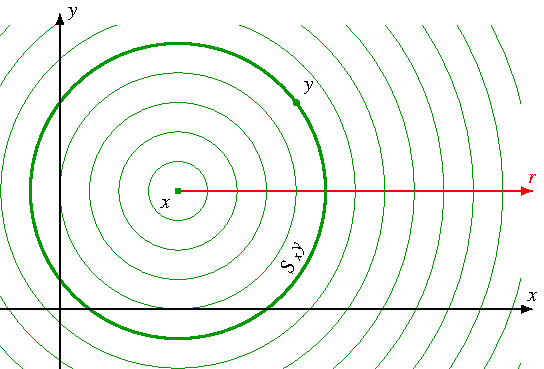
\includegraphics{chapters/070-nichtkomm/images/2dmendez.pdf}
\caption{Die Méndez-Transformation einer Funktion $f$ in der
Ebene an der Stelle $x,r$ ist der Mittelwert der Funktionswerte
auf auf dem Kreis $S_xy$ mit Radius $r=|y-x|$ um den Punkt $x$.
\label{buch:nichtkomm:mendez:fig:2d}}
\end{figure}
Für das Registrierungsproblem auf der Ebene mit der Gruppe
$\operatorname{SO}(2)\ltimes \mathbb{R}^2$ sind die Orbits des
Stabilisators eines Punktes $P=(x,y)$ Kreise vom Radius $r$ um
den Punkt (Abbildung~\ref{buch:nichtkomm:mendez:fig:2d}).
Der Raum $K\backslash G/K$ besteht aus den nichtnegativen
Zahlen $\mathbb{R}_{\ge 0}$.
Die Méndez-Transformation von $f$ hat daher die Werte
\[
\mathcal{M}f(P)(r)
=
\frac{1}{2\pi}
\int_0^{2\pi}
f(x+r\cos\varphi,y+r\sin\varphi)\,d\varphi.
\]
\end{beispiel}

\begin{beispiel}
Für das Registrierungsproblem auf der Kugeloberfläche ist $x$ irgend ein
Einheitsvektor.
Die Orbits des Stabilisators von $x$ sind die Breitenkreise bezüglich
der Achse der Kugel durch $x$.
Sie sind durch die Höhe über der zu $x$ orthogonalen Äquatorebene der
Kugel charakterisiert.
Die Méndez-Transformierte einer Funktion $f\colon S^2\to \mathbb{R}$
an der Stelle $x$ ist daher eine Funktion $[-1,1]\to\mathbb{R}$ mit
dem Wert
\[
\mathcal{M}f (x)(z)
=
\int_{S_x} f(k\tilde{z})\,dk,
\]
wobei $\tilde{z}$ ein Einheitsektor mit $\tilde{z}\cdot x=z$ ist.
Das Integral ist der Mittelwert von $f$ über den Breitenkreis
auf Höhe $z$ um die Achse $x$.
\end{beispiel}

Die Méndez-Transformation wurde von Tabea Méndez in 
\cite{buch:mendez} zur Lösung des Registrierungsproblems erfunden
und in \cite{buch:mendez-mueller} weiter verallgemeinert.
Die allgemeinste Darstellung der Theorie ist \cite[chapter 3]{buch:reg},
wo auch der Zusammenhang zur Radon-Transformation hergestellt wird.

%
% Lösung des Registrierungsproblems
%
\subsection{Lösung des Registrierungsproblems mit der Méndez-Transformation}
Es wurde bereits dargelegt, wie die Struktur des homogenen Raumes $G/K$
ermöglicht, das Registrierungsproblem in zwei einfachere Teilprobleme
zu zerlegen, nämlich das Finden eines Punktepaares, gefolgt von einem
Registrierungsproblem bezüglich der Gruppe $K$.
Mit der Méndez-Transformation kann der zweite Schritt jetzt vereinfacht
werden.
Wir zeigen hier nur das Prinzip, Optimierungsmöglichkeiten sind in
\cite{buch:mendez-mueller} und \cite{buch:reg} dargestellt.

%
% Registrierung mit einem Fixpunkt
%
\subsubsection{Registrierung mit einem Fixpunkt}
Falls die Wirkung der Gruppe $G$ auf $X$ immer einen Fixpunkt hat,
ist der erste Schritt des Registrierungsproblems besonders einfach
zu lösen.
In diesem Fall gibt es nämlich immer einen Punkt $x$, der beiden
Bildern gemeinsam ist.
Die Méndez-Transformationen $\mathcal{M}f(x)$ und $mathcal{M}g(x)$
sind daher die gleiche Funktion auf $Z=K\backslash G/K$.
Es muss daher nur der Definitionsbereich $X$ nach einem Punkt
durchsucht werden, für den $\mathcal{M}f(x) = \mathcal{M}g(x)$
gilt.
Da die Méndez-Transformation linear ist, bedeutet dies, dass nur
nach einer Nullstelle der Méndez-Transformation von $f-g$ gesucht
werden muss, also nach einem Punkt $x$, für den die Funktion
\(
\mathcal{M}(f-g)(x)
\)
die Nullfunktion ist.
Unter Berücksichtigung des Bildrauschens ist als $x$ so zu bestimmen,
dass die Norm $\| \mathcal{M}(f-g)(x) \|$ von $\mathcal{M}(f-g)(x)$
als Funktion auf $Z$ minimiert wird.

Das Registrierungsproblem auf der Kugeloberfläche gehört in diese
Klasse, den jede räumliche Drehung hat eine Drehachse, die fest
bleibt.
Das Finden eines Punktes mit $\mathcal{M}f(x)=\mathcal{M}g(x)$ 
kann immer noch eine ziemlich schwierige, nichtlineare Aufgabe sein.
Es ist aber nur noch ein zweidimensionales Problem, der Definitionsbereich
$S^2$ ist daher leichter zu durchsuchen als der dreidimensionale
Definitionsbereich $\operatorname{SO}(3)$.

Das Problem kann noch etwas vereinfacht werden durch die folgenden zwei
Beobachtungen, die in \cite{mendez-mueller} etwas vertieft besprochen
werden.
\begin{enumerate}
\item
Für beliebige stetige Funktionen $f$ und $g$ ist die
Mendez-Transformation auch nur eine stetige Funktion und die
Abhängigkeit von $x$ ist im allgemeinen nicht differenzierbar.
Die Funktion $\|\mathcal{M}(f-g)(x)\|$ kann daher stark verrauscht
sein und es kann schwierig sein, das Minimum zu finden.
Durch Glättung der Funktionen kann erreicht werden, dass $f$ und $g$
differenzierbar sind, so dass das Minimum leichter zu finden ist.
\item
Glättung hat ausserdem den Vorteil, dass $x\mapsto\|\mathcal{M}(f-g)(x)\|_2^2$
eine differenzierbare Funktion ist, so dass ein gemäss 1.~gefundenes
approximatives Minimum mit Hilfe des quadratisch konvergenten Newtonschen
Algorithmus schnell verbessert werden kann.
\end{enumerate}

Weitere Möglichkeiten, die Lösung eines Registrierungsproblems mit
Hilfe eines Least-Squares-Ansatzes zu verbessern, sind in
\cite[chapter 3]{buch:reg} dargestellt.

%
% Registrierung ohne Fixpunkte
%
\subsubsection{Registrierung ohne Fixpunkte}
Beim Registrierungsproblem in der Ebene ist es möglich, dass die
Lösung ein reine Translation ist, die ausser im Fall der trivialen
Translation keine Fixpunkte hat.
In diesem Fall bleibt nichts anderes, als ein Punktepaar $x$ und $y$
zu finden so, dass $\mathcal{M}f(x)$ und $\mathcal{M}g(y)$ als Funktionen
auf $Z=K\backslash G/K$ übereinstimmen.
Dies sieht auf den ersten Blick nach einem sehr viel aufwendigeren
Problem aus, weil der Raum aller Punktepaare der vierdimensionale
Raum $\mathbb{R}^2\times\mathbb{R}^2$ ist.
Zwei Einschränkungen zeigen aber, dass dies nicht wirklich die
Schwierigkeit ist.
\begin{enumerate}
\item
Praktische Registrierungsprobleme suchen nur nach einer Translation
über eine beschränkte Distanz, gegeben durch die endliche Grösse 
der beiden Bilder.
\item
In einem realistischen Registrierungsproblem gibt es meistens einen
bekannten Bildpunkt des ersten Bildes, von dem man weiss, dass er auch
im zweiten Bild irgendwo vorkommt.
Es muss jetzt also nur noch der entsprechende Punkt im zweiten Bild
gesucht werden, was das Problem auf ein zweidimensionales Problem
reduziert.
\end{enumerate}



